%! Author = sriadityavedantam
%! Date = 4/8/26

\section{Divisors}

Suppose $X$ is a quasi-projective irreducible variety.

\begin{definition}[Prime Divisor]
    A prime divisor on $X$ is an irreducible subvariety of $X$ of codimension $1$.
\end{definition}

If $X = \aa^1$ or $\pp^1$, then a prime divisor is a single point.
If $X$ is a surface, then a prime divisor is a curve.

\begin{definition}[Weil Divisor]
    A Weil divisor $D$ on $X$ is given by
    \[
        D = k_1C_1 + \ldots + k_rC_r,
    \]
    where $k_i\in \z$ and each $C_i$ is a prime divisor.
\end{definition}

We define
\[
    \Div(X) \coloneqq \left\{\sum k_i C_i : k_i\in \z,\ C_i \text{ prime divisors}\right\},
\]
which is an abelian group.
We define the \textbf{\textit{support}} of $D$ to be the union of all $C_i$.

\begin{definition}[Effective]
    A divisor $D$ is effective if $k_i \geq 0$ for all $i$, and not all $k_i$ are $0$.
\end{definition}

\begin{figure}[H]
    \centering
    \captionsetup{justification=centering}
    \tikzset{every picture/.style={line width=0.75pt}}

    \colorbox{white}{%
        \color{black}
        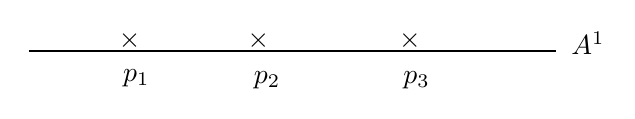
\begin{tikzpicture}[
            x=0.75pt,
            y=0.75pt,
            yscale=-1,
            xscale=1,
            every node/.style={text=black},
            every path/.style={draw=black},
            line width=0.75pt
            ]
            \draw    (181,137) -- (435,137) ;

            \draw (441,126.4) node [anchor=north west][inner sep=0.75pt]    {$\mathbb{A}^{1}$};
            \draw (358,126.4) node [anchor=north west][inner sep=0.75pt]    {$\times$};
            \draw (285,126.4) node [anchor=north west][inner sep=0.75pt]    {$\times$};
            \draw (223,126.4) node [anchor=north west][inner sep=0.75pt]    {$\times$};
            \draw (225,144.4) node [anchor=north west][inner sep=0.75pt]    {$p_{1}$};
            \draw (288,145.4) node [anchor=north west][inner sep=0.75pt]    {$p_{2}$};
            \draw (360,145.4) node [anchor=north west][inner sep=0.75pt]    {$p_{3}$};
        \end{tikzpicture}
    }
    \caption{Defining points for a divisor on $\aa^1$, \\
    for example the divisor $3p_1 - p_2 + 5p_3$.}
\end{figure}

Thus the corresponding rational function can be thought of as
\[
    \frac{f_1^3 f_3^5}{f_2}.
\]

\begin{figure}[H]
    \centering

    \tikzset{every picture/.style={line width=0.75pt}}

    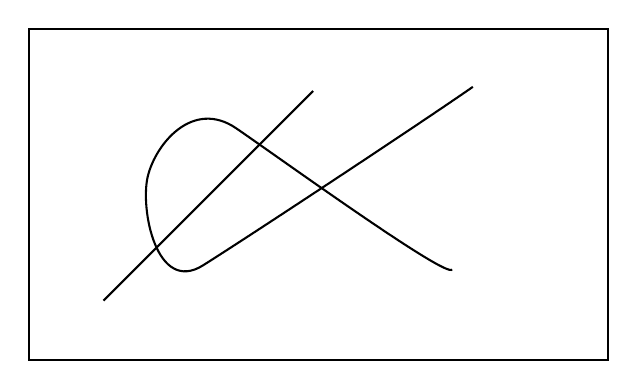
\begin{tikzpicture}[x=0.75pt,y=0.75pt,yscale=-1,xscale=1]
        \draw   (194,68) -- (473,68) -- (473,227.43) -- (194,227.43) -- cycle ;
        \draw    (398,184) .. controls (395.49,188.56) and (314.88,130.29) .. (294,116) .. controls (273.12,101.71) and (255.16,123.38) .. (251.36,139.16) .. controls (247.56,154.94) and (255.58,196.11) .. (278,182) .. controls (300.42,167.89) and (382.03,114.06) .. (408,96) ;
        \draw    (331,98) -- (230,199) ;
    \end{tikzpicture}

    \caption{All points on the line and curve.}
\end{figure}

We state our goal.
Given $f\in \c(X)\setminus\{0\}$, we define what $\div(f)\in \Div(X)$ is.
Assume $X$ is nonsingular in codimension $1$.
This means $\Sing(X)$ has codimension at least $2$, so in particular $X$ is normal.
Given $f$, we define the order of vanishing $\nu_C(f)$ along a prime divisor $C\subset X$.
Pick $U\subset X$ affine and dense such that $C\cap U \neq \varnothing$.
Then $C\cap U$ is a prime divisor of $U$, and since $U$ is normal, it is cut out by a prime element $\pi$ locally.

\begin{figure}[H]
    \centering

    \tikzset{every picture/.style={line width=0.75pt}}

    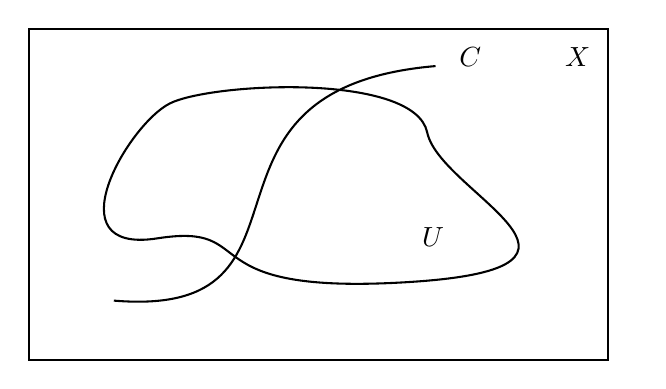
\begin{tikzpicture}[x=0.75pt,y=0.75pt,yscale=-1,xscale=1]
        \draw   (194,68) -- (473,68) -- (473,227.43) -- (194,227.43) -- cycle ;
        \draw   (262,104) .. controls (282,94) and (380,89) .. (386,118) .. controls (392,147) and (487,183) .. (378,190) .. controls (269,197) and (307,161) .. (256,169) .. controls (205,177) and (242,114) .. (262,104) -- cycle ;
        \draw    (235,199) .. controls (343,208) and (261,97) .. (390,86) ;

        \draw (451,75.4) node [anchor=north west][inner sep=0.75pt]    {$X$};
        \draw (382,162.4) node [anchor=north west][inner sep=0.75pt]    {$U$};
        \draw (400,75.4) node [anchor=north west][inner sep=0.75pt]    {$C$};
    \end{tikzpicture}
\end{figure}

Write
\[
    f|_U = \frac{g}{h}\in \c(U),
\]
with $g,h\in \c[U]$.
There is a unique integer $k\in \z_{\geq 0}$ such that $g\in (\pi)^k$ but $g\notin (\pi)^{k+1}$.
Then $k$ is the largest integer such that $\pi^k \mid g$.
We set $\nu_C(g) = k$.
Define similarly $\nu_C(h)$.
Finally set
\[
    \nu_C(f) \coloneqq \nu_C(g) - \nu_C(h).
\]
We remark that $\nu_C(f)$ is independent of the choice of $U$.
If $X = \aa^1$, then $\c(X) = \c(t)$.
Suppose
\[
    f(t) = \frac{(t+3)^2(t-2)}{(t+1)^4}.
\]
If nothing divides the numerator or denominator at a given point, then the order of vanishing there is $0$.
In this case, we can split $f(t)$ into factors and read off the order of vanishing at each point.
This leads to the definition of $\div(f)$.

\begin{proposition*}{
    For any $f\in \c(X)\setminus\{0\}$, there are only finitely many prime divisors $C$ such that
    \[
        \nu_C(f)\neq 0.
    \]
}
\end{proposition*}

\begin{definition}[Divisor of $f$]
    \[
        \div(f) \coloneqq \sum_C \nu_C(f)\,C,
    \]
    where the sum runs over all prime divisors $C$.
\end{definition}

\begin{definition}[Principal Divisor]
    A divisor $D\in \Div(X)$ is principal if there exists $f\in \c(X)\setminus\{0\}$ such that
    \[
        D = \div(f).
    \]
\end{definition}

For the $f$ above, we obtain
\[
    \div(f) = 2\{t = -3\} + \{t = 2\} - 4\{t = -1\}.
\]
In fact, any point on $\aa^1$ gives a principal divisor, but this is not true on $\pp^1$ unless we also account for the point at infinity.
We find this intuition by thinking of projective space as
\[
    \pp^1 = \aa^1_t \cup \aa^1_u,
\]
where $\infty = \{u = 0\}\subset \aa^1_u$.
For example,
\[
    \div(t) = \{t = 0\} - \{\infty\}.
\]
Equivalently,
\[
    \nu_{\{\infty\}}(t) = -1.
\]